\chapter{Поля волноводов}
\section{Поле на их границе}
Поле в волноводе в некотором приближении - это нормальное распределение. Формула зависимости от x и y 
выглядит вот так:
\begin{equation}
  \label{gauss2d}
  E(x,y)=\frac{1}{2\pi\sigma_1\sigma_2}\exp\left(-\frac{x^2}{2\sigma_1^2}-\frac{y^2}{2\sigma_2^2}\right)
\end{equation}
Таким образом мы получим нормальное распределение с вершиной в точке $(0,0)$
Волноводы разных конфигурраций возбуждают моды с разным распределением поля. Для сравнения, на рисунке показаны распределния поля цилиндрического и планарного волноводов

\noindent
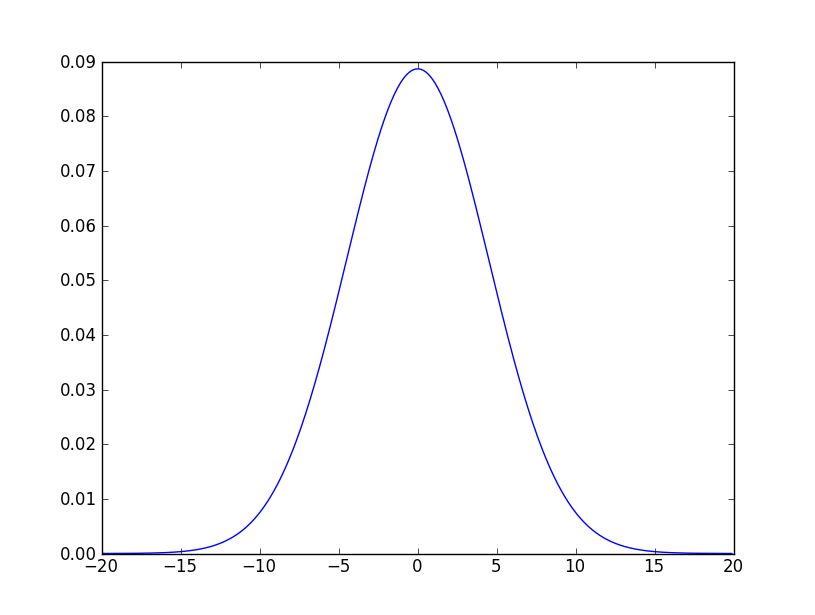
\includegraphics[width=0.5\textwidth]{img/cylinderGauss.png}
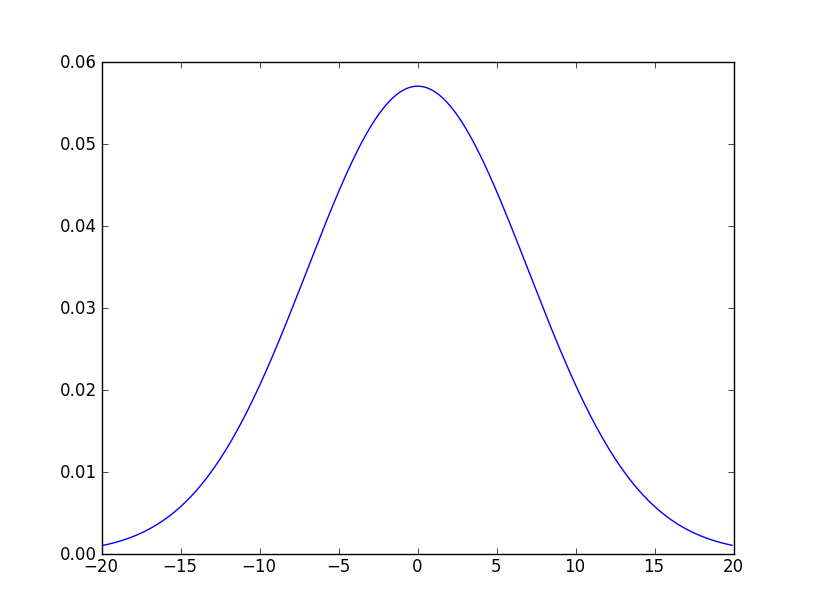
\includegraphics[width=0.5\textwidth]{img/planarGauss.png}

Здесь видно, что эти поля не совпадают, следовательно при их соединении перейдёт не вся энергия, а только та часть, которая перекрывается обоими распределениями

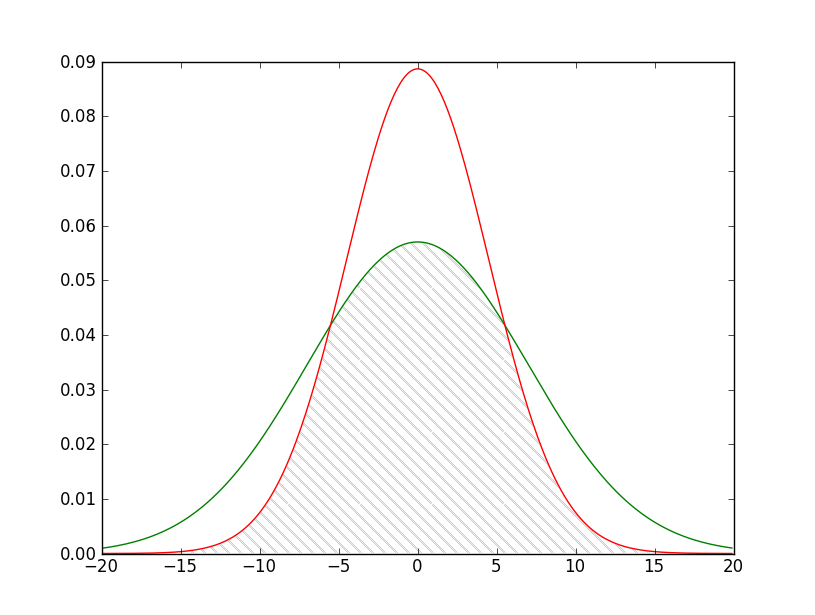
\includegraphics[width=0.5\textwidth]{img/intersection.png}

В случае, если волноводы совмещены не соосно, то площадь перекрытия уменьшается еще больше:

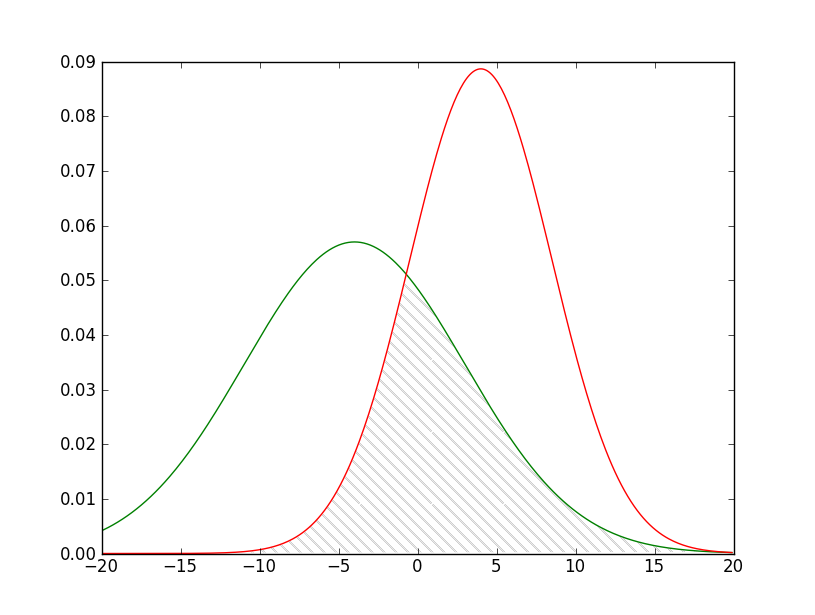
\includegraphics[width=0.5\textwidth]{img/intersection2.png}

\section{Объяснение зависимости}

